\section{Conclusion}

\subsection{Wave Interpretation}
It was expected that $H/S_{msr} - H/S_{thm}$ data had a best-fit line of the slope of 1 at high frequency. As $\omega$ increases, $z$ increases (Equation \ref{dispersion_relation}) and $H/S$ decreases (Equation \ref{eq_023}), so the linear trend was expected to be more definite at low $H/S$. With $\omega < 2\pi$ ($H/S_{thm} < 1$), a linear trend was apparent with the best-fit line of $y=0.5773x$ and $R^{2} = 0.9928$. Though it had a linear trend with high precision, the slope wasn't 1.0000, and the number of data was insufficient. 

The plate moved in the fine sinusoidal waveform at low $\omega$, such as Figure \ref{Data_omega=3_plate} (c) and (d). Corresponding wave height data (Figure \ref{Data_omega=4_plate} (c) and (d)) had a small peak at the position of the trough, which means that the reflected wave was not negligible. This phenomenon was constant in some cases with $\omega=6.0$ such as Figure \ref{Data_omega=6_wave} (c) and (d). As $A$ increased, more small peaks were observed.

As $\omega$ increased, the motor malfunctioned. It was quite definite in Figure \ref{Data_omega=6_plate} (e) and (f). It was mainly due to the impulse exerted by fluid flow, and the wave absorber needed improvement. The effect of reflective wave could be seen from small peaks in Figure \ref{Data_omega=6_wave} (e), (f), and so on. Motor malfunctioned more critically at higher $\omega$. With $\omega\geq7$, the plate oscillated side to side, and the center of oscillation also moved with a scale similar to the amplitude of oscillation. Though the plate displacement was not a proper sinusoidal, sin-like wave were created (Figure \ref{Data_omega=7_wave}, \ref{Data_omega=9_wave}, \ref{Data_omega=}). 

Considering that the wavemaker was built as lab equipment, calibration is needed regardless of relevant theories. But one thing was definite, that to generate a sinusoidal wave, high $\omega$ was demanded.

Also, the theoretical approach was not sufficient to conclude the experimental result. Though a wave absorber was installed, reflected waves existed, and the wavemaker theory of Dean and Dalrymple required ideal conditions and approximations \cite{dean1991water}. Considering the reflection and second order of $\phi$, the wave function could be written as in \cite{madsen1971generation}. It's based on Stokes wave theory, and the wave function is expressed as the following.
\begin{equation}
    \eta = -a \left[ \sin{(kx - \omega t)} + \epsilon_{p} \left[\cos{2(kx - \omega t)} - \cos{(kx - 2\omega t)}\right] + O(\epsilon_{p}^{2}) \right]
    \label{Madsen1971}
\end{equation}

Though the equation is given, the wave height recorded from the buoy and analyzed with FFT and curve fitting was measured with fixed $x$, which is not tolerable as a wave form given from \cite{madsen1970waves}.

\subsection{Limitation}

In conclusion, the wavemaker can generate proper short waves with parameters, though there were limits. To generate a short wave with given $H$ and $\sigma$, $S_{0}$ should be calculated to determine if the motor can move with it. Also, $A$ must be known: as it was said, there had been no apparent relation between $A$ and $S_{0}$, and further calibration is required.

\begin{figure}[H]
    \centering
        \begin{filecontents}{acc.dat}
                t	y_30000	y_40000	y_50000
                0	0.19965	-0.0461	-0.70283
                0.033367	0.88578	0.79731	0.26519
                0.066734	1.41854	1.54643	1.3542
                0.1001	1.78019	2.09436	2.16649
                0.133467	2.10058	2.51832	2.74721
                0.166834	2.42496	2.9166	3.28632
                0.2002	2.65052	3.25279	3.73685
                0.233567	2.69128	3.32493	3.95223
                0.266934	2.69601	3.32011	4.0169
                0.3003	2.68381	3.31722	4.04341
                0.333667	2.53945	3.18505	3.92908
                0.367034	2.24984	2.85109	3.62093
                0.4004	1.94568	2.46075	3.19471
                0.433767	1.6103	2.00279	2.6843
                0.467134	1.14521	1.38601	1.98441
                0.5005	0.55864	0.64207	1.11098
                0.533867	-0.0586	-0.14149	0.16794
                0.567234	-0.68693	-0.94865	-0.8004
                0.6006	-1.16272	-1.669	-1.63958
                0.633967	-1.51151	-2.20274	-2.34206
                0.667334	-1.86959	-2.67197	-3.00563
                0.7007	-2.15706	-3.05802	-3.48397
                0.734067	-2.2686	-3.25109	-3.80335
                0.767434	-2.3295	-3.3759	-4.05893
                0.8008	-2.3925	-3.44363	-4.18022
                0.834167	-2.34221	-3.34345	-4.09689
                0.867534	-2.12824	-3.09611	-3.91013
                0.9009	-1.92868	-2.80851	-3.63691
                0.934267	-1.66742	-2.44389	-3.16259
                0.967634	-1.20691	-1.87777	-2.55154
                1.001	-0.71952	-1.22286	-1.84435
                1.034367	-0.20613	-0.50127	-1.04396
                1.067734	0.42368	0.31501	-0.09588
                1.1011	1.05093	1.12604	0.91296
                1.134467	1.51691	1.75337	1.7925
                1.167834	1.85038	2.20687	2.43867
                1.2012	2.15589	2.58406	3.00982
                1.234567	2.44035	2.96622	3.51607
                1.267934	2.55892	3.18147	3.8099
                1.3013	2.58132	3.1805	3.92574
                1.334667	2.58654	3.18082	3.99092
                1.368034	2.50032	3.12393	3.96888
                1.4014	2.27759	2.85251	3.70347
                1.434767	2.01037	2.44489	3.35212
                1.468134	1.70864	2.02859	2.9192
                1.5015	1.27966	1.48942	2.28589
                1.534867	0.72957	0.7975	1.52725
                1.568234	0.13968	-0.00332	0.65856
                1.6016	-0.46007	-0.82565	-0.34092
                1.634967	-1.00343	-1.61238	-1.27387
                1.668334	-1.39078	-2.12874	-1.98071
                1.7017	-1.73618	-2.63824	-2.67774
                1.735067	-2.05872	-3.06711	-3.25502
                1.768434	-2.2378	-3.33038	-3.59615
                1.8018	-2.28124	-3.46167	-3.88219
                1.835167	-2.35317	-3.55984	-4.08709
                1.868534	-2.34231	-3.52169	-4.05134
                1.9019	-2.18136	-3.3411	-3.88661
                1.935267	-1.96749	-3.06891	-3.67773
                1.968634	-1.71625	-2.72452	-3.26969
                2.002	-1.28602	-2.2191	-2.70558
                2.035367	-0.81728	-1.55728	-2.02746
                2.068734	-0.31872	-0.84745	-1.2709
                2.1021	0.26265	-0.07845	-0.30425
                2.135467	0.9496	0.788	0.72003
                2.168834	1.40154	1.52533	1.62134
                2.2022	1.75468	2.01573	2.30078
                2.235567	2.10147	2.46746	2.94581
                2.268934	2.3967	2.87079	3.47737
                2.3023	2.55238	3.15844	3.81726
                2.335667	2.62076	3.23622	4.00602
                2.369034	2.65914	3.27771	4.14932
                2.4024	2.58367	3.24675	4.15548
                2.435767	2.39857	3.05535	3.94408
                2.469134	2.17446	2.71809	3.62721
                2.5025	1.88444	2.34949	3.25509
                2.535867	1.49925	1.85688	2.65401
                2.569234	1.00332	1.21929	1.93541
                2.6026	0.44518	0.50017	1.14535
                2.635967	-0.19936	-0.3095	0.13966
                2.669334	-0.74776	-1.08519	-0.83255
                2.7027	-1.20231	-1.64584	-1.61405
                2.736067	-1.59977	-2.20759	-2.37864
                2.769434	-1.93983	-2.65238	-3.00176
                2.8028	-2.17932	-2.94288	-3.4264
                2.836167	-2.29458	-3.10488	-3.73815
                2.869534	-2.37942	-3.21108	-3.99138
                2.9029	-2.38288	-3.20642	-4.04015
                2.936267	-2.27697	-3.0282	-3.91074
                2.969634	-2.1216	-2.7839	-3.74705
                3.003	-1.91887	-2.45772	-3.3983
                3.036367	-1.55399	-1.99512	-2.917
                3.069734	-1.07152	-1.35359	-2.28586
                3.1031	-0.64736	-0.69868	-1.56226
                3.136467	-0.07503	0.07567	-0.67443
                3.169834	0.62139	0.96725	0.30019
                3.2032	1.15329	1.72133	1.32913
                3.236567	1.52816	2.28082	2.12527
                3.269934	1.89348	2.70848	2.72048
                3.3033	2.24371	3.18353	3.26412
                3.336667	2.43633	3.40231	3.70057
                3.370034	2.53906	3.47484	3.94051
                3.4034	2.60009	3.55977	4.05245
                3.436767	2.56799	3.57702	4.09095
                3.470134	2.42036	3.37121	3.96946
                3.5035	2.20923	3.07584	3.65483
                3.536867	1.93066	2.78252	3.2648
                3.570234	1.55913	2.26567	2.78462
                3.6036	1.10325	1.61979	2.07279
                3.636967	0.5802	0.97997	1.24147
                3.670334	-0.02334	0.17924	0.34297
                3.7037	-0.65857	-0.75173	-0.64667
                3.737067	-1.17285	-1.37792	-1.55053
                3.770434	-1.56799	-1.91885	-2.26503
                3.8038	-1.90164	-2.46202	-2.94488
                3.837167	-2.23698	-2.85342	-3.50423
                3.870534	-2.44391	-3.05384	-3.83199
                3.9039	-2.49569	-3.19402	-4.0644
                3.937267	-2.51034	-3.29516	-4.2654
                3.970634	-2.5445	-3.24324	-4.26093
                4.004	-2.42687	-3.03	-4.03252
                4.037367	-2.16947	-2.75013	-3.75746
                4.070734	-1.90945	-2.413	-3.36757
                4.1041	-1.51816	-1.933	-2.83599
                4.137467	-1.03935	-1.29424	-2.10184
                4.170834	-0.50818	-0.57231	-1.2709
                4.2042	0.06957	0.31284	-0.26666
                4.237567	0.73165	1.17361	0.75584
                4.270934	1.2455	1.87399	1.6875
                4.3043	1.58747	2.36544	2.40174
                4.337667	1.89112	2.73069	2.95997
                4.371034	2.16959	3.11726	3.35944
                4.4044	2.37204	3.38282	3.71815
                4.437767	2.4319	3.40654	3.89543
                4.471134	2.42094	3.3675	3.95554
                4.5045	2.3439	3.3302	3.92504
                4.537867	2.18696	3.1265	3.74224
                4.571234	1.92323	2.7545	3.39073
                4.6046	1.59431	2.28924	2.94849
                4.637967	1.21345	1.74871	2.39218
                4.671334	0.71115	1.12462	1.6625
                4.7047	0.12966	0.3269	0.79821
                4.738067	-0.47148	-0.51087	-0.16585
                4.771434	-1.05047	-1.27666	-1.12757
                4.8048	-1.49682	-1.80115	-1.92418
                4.838167	-1.82838	-2.27316	-2.58851
                4.871534	-2.17445	-2.71807	-3.17688
                4.9049	-2.43635	-3.04975	-3.62932
                4.938267	-2.48784	-3.21874	-3.86814
                4.971634	-2.51503	-3.29405	-4.06024
                5.005	-2.56856	-3.30492	-4.15906
                5.038367	-2.4869	-3.1784	-4.04501
                5.071734	-2.25169	-2.91066	-3.74639
                5.1051	-2.01171	-2.55853	-3.3832
                5.138467	-1.7465	-2.1082	-2.98582
                5.171834	-1.28108	-1.54368	-2.3775
                5.2052	-0.75679	-0.94807	-1.61234
                5.238567	-0.19342	-0.15545	-0.61791
                5.271934	0.41501	0.72147	0.35113
                5.3053	0.97708	1.50741	1.32609
                5.338667	1.38601	2.09393	2.13243
                5.372034	1.69529	2.46928	2.73626
                5.4054	1.9505	2.84432	3.30207
                5.438767	2.13855	3.19731	3.73049
                5.472134	2.23725	3.34286	4.02161
                5.5055	2.25088	3.2946	4.16939
                5.538867	2.18332	3.24129	4.16521
                5.572234	2.03225	3.17057	4.03556
                5.6056	1.80633	2.85472	3.7849
                5.638967	1.50978	2.36769	3.37659
                5.672334	1.12638	1.89813	2.83644
                5.7057	0.61015	1.3599	2.17771
                5.739067	0.09032	0.56945	1.35831
                5.772434	-0.51844	-0.26237	0.43367
                5.8058	-1.17384	-1.05176	-0.52577
                5.839167	-1.65163	-1.76004	-1.41355
                5.872534	-1.99282	-2.29776	-2.09461
                5.9059	-2.39362	-2.74567	-2.7724
                5.939267	-2.69534	-3.09648	-3.28198
                5.972634	-2.83697	-3.30478	-3.59474
                6.006	-2.97469	-3.43862	-3.80204
                6.039367	-3.04448	-3.47008	-3.97475
                6.072737	-2.96871	-3.40402	-3.96754
                6.106097	-2.80123	-3.19323	-3.7299
                6.139467	-2.578	-2.91812	-3.37793
                6.172837	-2.32669	-2.54115	-3.01313
                6.206197	-2.02032	-2.05056	-2.49922                    
            \end{filecontents}
        
            \begin{tikzpicture}[
                    %Environment Cfg.
                    font=\bfseries\sffamily,
                ]
                    \begin{axis}[
                        width=\textwidth,
                        height=8cm,
                        at={(0,0)},
                        ymin=-4.3,
                        ymax=4.3,
                        xmin=0,
                        xmax=7,
                        grid=both,
                        minor tick num =5,
                        minor tick style={draw=none},
                        minor grid style={thin,color=black!10},
                        major grid style={thin,color=black!10},
                        %ylabel style={rotate=90},
                        ylabel={$y~\left[\mathrm{cm} \right]$},
                        xlabel={$t~\left[\mathrm{s} \right]$},
                        tick align=outside,
                        axis x line*=middle,
                        axis y line*=none,
                        xtick={0, 2, 4, 6, 8},
                        ytick={-4, -2, 0, 2 ,4},
                        %xlabel style={color=blue!50!cyan},
                        %ylabel style={align=center,rotate=-90,color=blue!50!cyan},
                        x tick label style={
                            /pgf/number format/assume math mode, font=\sf\scriptsize,
                            % yshift={-mod(\ticknum,1)*7em}
                            yshift=.5*\axisdefaultheight
                            % yshift = {7em}
                            },
                        y tick label style={
                            /pgf/number format/assume math mode, font=\sf\scriptsize},
                        legend cell align = {left},
                        % legend pos = north east,
                        legend style={at={(1,1)},anchor=north east},
                        legend style={nodes={scale=0.5, transform shape}},
                        ]
                        %\addplot [only marks, mark = *] table [x=t, y_30000, y_40000, y_50000] {acc.dat};
                        \addplot [%only marks, 
                            mark = +,
                            mark size=1.5pt,
                            color=black,
                            ] 
                            table [x=t, y=y_30000] {acc.dat};
                        \addlegendentry{acc = 30000};
                        \addplot [%only marks, 
                            mark = *,
                            mark size=1.5pt,
                            color=black,
                            ] 
                            table [x=t, y=y_40000] {acc.dat};
                        \addlegendentry{acc = 40000};
                        \addplot [%only marks, 
                            mark = o,
                            mark size=1.5pt,
                            color=black,
                            ] 
                            table [x=t, y=y_50000] {acc.dat};
                        \addlegendentry{acc = 50000};
                        % \addplot[color=blue!50!cyan,smooth,tension=0.7,very thick] table [x index=0,y index=1,col sep=space] {Aplate-wmsrS.dat};
                        % \addplot[color=cyan!50!lime,very thick] coordinates{(0,5)(25,5)};
                        % \addplot[color=orange,very thick] coordinates{(0,11)(25,11)};
                        % \addplot[color=red!80!orange,very thick] coordinates{(19,24.2)(23,24.2)};
                        % \node[text=cyan!50!lime,fill=white,align=center,anchor=west,scale=0.8,inner sep=5pt] at (24.5,5){Base\\ Load};
                        % \node[color=orange,fill=white,align=center,anchor=west,scale=0.8,inner sep=5pt] at (24.5,11){Average\\ Load};
                        % \node[color=red!80!orange,fill=white,align=center,anchor=west,scale=0.8,inner sep=5pt] at (21.2,24.2){Maxium\\ Load};
                    \end{axis}
        \end{tikzpicture}
    \caption{Waveheight graph (variation of MaxAcceleration)}
    \label{Experiment(Acceleration)}
\end{figure}

MaxAcceleration was one factor that affected the performance of the motor. Figure \ref{Experiment(Acceleration)} shows differing movement of the plate under the condition of \textit{MaxAcceleration} = $30,000, ~40,000$ and $50,000 \mathrm{~step/s^{2}}$. As the \textit{MaxAcceleration} increased, the amplitude of the wave increased which means that the velocity could be changed more rapidly with a bigger difference, giving out better(more precise) output.

Also, the malfunction of the step motor was critical. It 

\subsection{Improving Experimenting System}
The wave channel and the whole experimenting system need a lot of improvements (wavemaker, wave channel, wave gauge, and wave absorber). Still, there are several parameters more than $A$ and $\omega$ - $N$, the number of steps and current(from the motor driver), MaxSpeed, MaxAcceleration, etc. - that play a role in the code, and a better understanding of the wavemaker is necessary. Due to the limited time, a fundamental experiment involving only $A$ and $\omega$ had been conducted in this paper, but other parameters could be able to help out making more delicate waves.

Also, the performance of the wave absorber needs testing. Currently, baskets with holes, filled with scrubbers are used as the wave absorbers. The structure of it (the size, number, and orientation of the holes) could be standardized, and comparing various structures can be another research. Moreover, the coastal model is variable and it can be shifted to install other structures on the flat land. A model wave power can be placed here so that various types can be compared at certain conditions.

Lastly, a proper wave gauge was needed. Using a buoy was a fine idea, but it was impaired by several waves and had an intrinsic error of rotating. Also, it was fixed horizontally, so that collecting wave height throughout the wave channel was inappropriate. A new type of wave gauge was in need, that can collect data and interpret is to wave height as soon as it was measured. In the case of the buoy, the whole system must be changed so that as soon as the video is recorded, the location of the buoy is recorded.

% \begin{figure}[htbp]
%     \centering
%     \includegraphics[height=5.5cm]{images/Breakwater.jpg}
%     \includegraphics[height=5.5cm]{images/Breakwater(Illustrated).jpg}
%     \caption{방파제 모형(왼쪽)과 규격(오른쪽)}
%     \label{Braekwater}
% \end{figure}

% 규격 $D3=1.2\mathrm{~cm}, D2=1.7\mathrm{~cm}, S=5.3\mathrm{~cm}, F=5\mathrm{~cm}$의 방파제 모형을 이용한 연구를 진행할 예정이다. 방파제의 조적 구조는 Gurer의 구조, Fabiao의 구조 등 여러 종류가 있으며 구조의 종류 및 스케일에 대한 방파 효과를 비교할 수도 있다\cite{article}.
%참고문헌 필요함.

\subsection{Generating Irregular Wave}
The ultimate goal of the wavemaker is to provide proper environments for model experiments. In the case of a piston-type wavemaker, irregular waves could be generated by changing its movement or the plate. Changing the plate means that the plate is divided into small pieces and each piece moves with its signal. This wavemaker is called snake-like, and it's illustrated in Figure \ref{Snake Wave Maker}.

\begin{figure}[H]
    \centering
    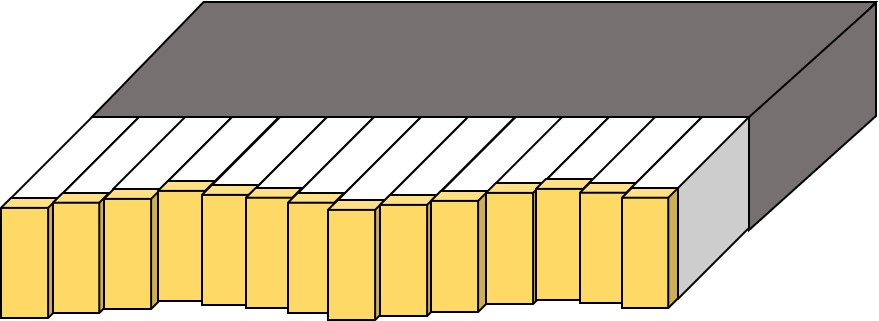
\includegraphics[width=10cm]{images/Wave_Maker(Snake).jpg}
    \caption{3-dimensional wavemaker(snake-like)}
    \label{Snake Wave Maker}
\end{figure}

In other words, the 3-dimensional wavemaker is needed. Though it's not 3-dimensional, the signal provided to the motor could be modified. In a special case, a tsunami could be generated \cite{watts1998wavemaker}.
 
